\documentclass[a4paper,12pt]{article}
\usepackage[utf8x]{inputenc}
\usepackage{ucs}
\usepackage[czech]{babel}
\usepackage[T1]{fontenc}
\usepackage[left=3.5cm,right=2cm,top=3cm,bottom=3cm]{geometry}

\usepackage{amsmath,amsfonts,amssymb}
\usepackage{gensymb,marvosym}
\usepackage{times}
\usepackage{tabularx}
\usepackage{graphicx}

% More rows in one table (one row as multiple rows)
\usepackage{multirow}

% Dotted line for a signature
\usepackage{arydshln}

\usepackage[none]{hyphenat} \sloppy
\clubpenalty 10000
\widowpenalty 10000

% Declaring for the use of coloured boxes
%\usepackage{xcolor}
%\usepackage{mdframed}
\usepackage{framed}

% Line space settings
\usepackage{setspace} \onehalfspacing

\usepackage{enumerate}

% === Setting up main parameters ===
\newcommand{\autor}{Dominik Bálint}           % <-- Author
\newcommand{\skola}{CEVRO Institut}           % <-- Univerzity
\newcommand{\fakulta}{Právo v obchodních vztazích}         % <-- Faculty
\newcommand{\nazev}{Dezinformace ve světle světové pandemie, jiných nemocí a vakcinace}           % <-- Title
\newcommand{\typPrace}{Seminární práce}        % <-- Paper type
%\newcommand{\vedouciPrace}{}    % <-- Lead

% PDF metadata setting
\usepackage[pdftex,
            pdfauthor={dominikbalint},                  % <-- PDF Author
            pdftitle={disinformace\_ve\_svetle\_svetove\_pandemie},                   % <-- PDF Title
            pdfsubject={},                      % <-- PDF Subject
            pdfkeywords={},                     % <-- PDF Keywords
            pdfproducer={CEVRO Institut},           % <-- PDF Producer
            pdfcreator={pdflatex}]{hyperref}    % <-- PDR Creator

\hypersetup{
    colorlinks = false,
    hidelinks
}

\usepackage{fancyhdr}
\usepackage{graphicx}

% Image folder location
\graphicspath{{pics/}}

% Charts package
\usepackage{float}
\newfloat{graf}{hbtp}{ext}
\floatname{graf}{Graf}

% Image names
\usepackage{caption}
\captionsetup[figure]{name=Obr.}

% ===
% Used to include url in BibTeX, more here: http://www.fit.vutbr.cz/~martinek/latex/czechiso.html
\usepackage{url}
\DeclareUrlCommand\url{\def\UrlLeft{<}\def\UrlRight{>} \urlstyle{tt}}

% Declaring trademark symbols
\usepackage{textcomp}
% ===

% === Beginning of the body of the document ===
\begin{document}
\pagestyle{empty}

\begin{titlepage}
	\centering

  \vfill

	{\LARGE \skola \par}
	{\Large \fakulta \par}

	\vfill

	{\huge\bfseries \nazev \par}
	{\Large \typPrace \par}

  \vfill

  {\Large Vedoucí práce: \vedouciPrace \par}
	{\Large Autor práce: \autor \par}

	\vspace{1.5cm}

	{\scshape\large Praha \the\year \par}

  \vfill
\end{titlepage}


\clearpage

% === File contents setting ===
% Table of contents
\tableofcontents

% Table of abbreviations
% Generally if you have more than five
% \section*{Seznam použitých zkratek}
\begin{tabularx}{\textwidth}{l X}
MIT licence          & Svobodná licence, která vznikla na Massachusettském technologickém institutu.
\end{tabularx}


% List of tables
% Generally if you have more than three tables
%\newpage
%\listoftables
%\thispagestyle{empty}

% List of images
% Generally if you have more than three images
\newpage
\listoffigures
\thispagestyle{empty}

\newpage

% Page numbering setting
\setcounter{page}{1}
\thispagestyle{empty}
%\pagestyle{empty}

% === Page header and page footer settings ===
\pagestyle{fancy}
\renewcommand{\headrulewidth}{0.5pt} %bez linky v zahlavi
\renewcommand{\footrulewidth}{0pt} %linka v zapati
\lhead{\leftmark}       \chead{} \rhead{} %pole zahlavi (prazdna)
\lfoot{} \cfoot{} \rfoot{\thepage} %pole zapati

% Including files containing your data, you can add more by defining new \include and creating a .tex file with the same name
\section*{Úvod}
Pravdou je, že v moderním světě je mnoho problémů, které můžeme vnímat jako bezpečností hrozbu. Jednou z nejskloňovanějších hrozeb v očích odborníků jsou v moderní \textit{post-truth} době dezinformace, ty jsou v rámci momentálně stále probíhající světové pandemie silnou zbraní, prostřednictvím které je možné ovlivnit veřejné mínění, názory a v konečném důsledku tedy i samotné chování jednotlivých lidí. Mnoho subjektů, ať už se jedná o individua, větší skupiny, či dokonce národní/nadnárodní skupiny, které mohou být nezřídkakdy podporovány i státy, se prostřednictvím dezinformací snaží dosáhnout svých cílů nejen na scéně domácí, ale i v zahraničí. Považuji proto za velice důležité o dezinformacích mluvit a zasadit se za osvětovou kampaň, aby proti snaze o použití dezinformací lidé byli více imunní. I z toho důvodu jsem se rozhodl pojednat ve své seminární práci o tématu dezinformací, a to specificky ve světle momentální pandemické situace, práce je tedy zaměřena především na dezinformace spojené s pandemií koronaviru a snahou o jeho zvládnutí (zde se dá hovořit například o dezinformacích směřovaných vůči vakcínám).

\section{Pojem dezinformace}

V moderní době internetové, kdy má přibližně 51\% obyvatel přístup k internetu\cite{noauthor_individuals_nodate}, se mohou dezinformace šířit stejnou rychlostí jako pravdivé informace a mnoho lidí tedy může snadlo podlehnout pocitu, že informace, které čtou, opravdu pravdivé jsou i když se ve skutečnosti jedná o dezinformace. Lze rovněž důvodně předpokládat, že v současné době, kdy mnoho lidí tráví více času doma než obvykle, bude dopad dezinformací značně větší.\\

Než ale přejdu k problematice dezinformací, je potřeba tento pojem nejdříve definovat. Pokud je třeba definovat jakýkoliv pojem, obracím se často na \textit{Oxford dictionary}, učinil jsem tak proto i teď, Oxfordský slovník dezinformace definuje jako: \textit{"false information that is given deliberately"}\cite{noauthor_disinformation_nodate}, v překladu tedy jako \textit{"nepravdivá informace, která je sdělena záměrně}.\\

V této souvislosti je nutné zmínit dvě "podkategorie" dezinformací, které je třeba vnímat odlišně, a to výše definovanou dezinformaci jakožto úmyslně nepravdivou informaci a dále "misinformaci", či špatnou informaci, která je neúmyslně šířena i když je nepravdivá (chybí tedy aspekt úmyslu sdílet špatnou informaci), nicméně to nic nemění na faktu, že je stále sdílena nepravdivá informace, což v konečném důsledku může vést k úplně stejným výsledkům\cite{lam_library_nodate}.\\

Nakonec je potřeba řící, že dezinformace nejsou ničím novým, existují již po celá milénia, nicméně v období před masovým využíváním internetu měly pouze omezený dosah. Postupné zvyšování dostupnosti moderní výpočetní techniky společně s internetem jako takovým umožnilo exponenciální nárůst v olbasti efektivnosti a množství šířených dezinformací. Dá se předpokládat, že k nárůstu šíření dezinformací přispělo především velké množství sociálních sítí, které umožnilo propojení lidí s podobnými zájmy napříč celým světem. Tento fakt ve svém důsledku umožnil subjektům, kteří chtějí dezinformace šířit, spojení s jinými subjekty s podobnými hodnotami, což v konečném důsledku dále zrychluje šíření dezinformací a zároveň v ně podporuje u těchto subjektů víru, neboť "nejsou sami, kdo si to myslí". Sociální sítě tak mají velkou možnost ovlivňovat celospolečenskou situaci jak v pozitivním, tak i v negativním světle, neboť jejich prostřednictvím je možné přispívat k diskuzi o směřování společnosti a rovněž i k vnímání jednotlivých témat ze strany společnosti.

\subsection{Dezinformace v době Covidové}

Jednou z největších výzev v době probíhající pandemie COVID-19 byl, je a bude nejen boj proti koronaviru jako takovému, ale i proti dezinformacím, které jsou využívány pro šíření nepravd či polopravd. Ve veřejném prostoru je možné sledovat mnoho diskuzí nad tím, jak se s dezinformacemi vypořádat.\\

Zdroje informací, a to jak v online prostoru, tak i v rámci televizního a rádiového vysílání, či dokonce v tisku jsou protkané nespočetným množstvím falešných a zavádějících tvrzení týkajích se zdroje, způsobu přenášení, závažnosti a v konečném důsledku i léčby viru a snahy o jeho vymícení. Může se jednat o poměrně neškodná marketingová tvrzení ohledně zdánlivě účinných produktů, jako například produkt od UVLEN \textregistered Technologies Korea\cite{uvlen__uvlen_nodate}, u kterého výrobce tvrdí, že má vlastnosti, které odporují základním zákonům fyziky (vlnovou délku světla není možné změnit za pomocí jednoduchého filtru), až po vážné útoky na vědce a orgány veřejné moci, které mohou vyůstit až v občanskou neposlušnost, jako příklad je možné připomenout nedávný útok na Kapitol zfanatizovaných davem, který se nechal přesvědčit dezinformacemi vyslovenými americkým prezidentem Donaldem Trumpem.\\

V této souvislosti je problémem právě to, že některé z těchto misinformací a dezinformací jsou širší veřejností opravdu považovány za pravdivé a to ať už jsou šířeny úmyslně (v případě dezinformací), či neúmyslně (v případě misinformací). Problémem u obou druhů dezinformací zůstává, že jsou stejně tak dobře schopny klamat a způsobovat újmu. Dezinformace představují pro společnost vážný problém, neboť podkopávají důvěru veřejnosti a zároveň díky svému nadměrnému množství znesnadňují schopnost dohledávat si pravdivé informace a důvěryhodné zdroje. Toto je obzvláštně nebezpečné v období pandemické krize, neboť mnoho dezinformací cílí na podkopání důvěry v protiepidemické opatření, zdravotní systém a očkování (u očkování je nechuť s ním spojená velice výrazná, přičemž argumenty "odmítačů" stojí převážně na nepravdivých informacích).\\ % Udělat vícuc jak lidi mluví o odmítání očkování na Twitteru

WHO problém s dezinformacemi zaměřující se na pandemii koronaviru označuje jako \textit{infodemii} a klade velký důraz na boj proti ní\cite{noauthor_covid-19_nodate}. V této souvislosti pak stanovuje dva velice důležité body v rámci boje proti dezinformacím:

\begin{enumerate}
\item nutnost zjistit, jak se dezinformace šíří,
\item nutnost vydefinovat způsob, jakým by na dezinformace měly světové vlády a korporace reagovat.	
\end{enumerate}

%\newpage

Způsob, jak proti dezinformacím bojovat práce načrtává v kapitole 3, nicméně již v této části práce je nutné řící, že reakce, jakožto bod druhý v řetězci řešení problému s dezinformacemi vyžaduje znalosti o bodu prvním, aby bylo možné navrhnout funkční způsoby určené právě k tomu, jak s dezinformacemi bojovat.\\

%\subsection{Studie, sdílení dezinformací prostřednictvím Twitteru}
%\subsection{Google Trends a dezinformace}

\section{Zdroje dezinformací, aneb jak se dezinformace šíří}

Misinformace a dezinformace bují nejvíce v dobách krizí a nejistot, dezinformace týkající se zdraví tedy bují nejvíce v dobách krize, která se zdraví obyvatel přímo týká, neboť se jedná o situace, ve kterých jsou obyvatelé znepokojení a bojí se dopadu na svoje vlastní zdraví a blahobyt. Je asi nasnadě říci, že právě v takové situaci se momentálně nacházíme. Přesně v takovýchto situacích je žízeň po zázračném léku, který nemoc přes noc vymítí, či po ujištění, že vlastně žádná krizová situace neexistuje, největší a dezinformace tak mají nejvíce prostoru k pronikání do našich \textit{news feedů} a k našemu následnému ovlivňování.\\

O závažnosti tohoto tématu svědčí i fakt, že na toto téma je v poslední době vypracováno mnoho studií, které se zabívají právě body stanovenými v kapitole 1, tedy zdrojem dezinformací a potenciálními přístupy k této problematice, respektive k jejímu řešení. Zajímavou studií týkající se problematiky je \textit{Types, sources, and claims of COVID-19 misinformation} od Dr. J. Scott Brennen a kol. z Reuters Institute for the Study of Journalism and the Oxford Internet Institute\cite{noauthor_types_nodate}, která poskytuje pohled na nynější alarmující informační stav ve společnosti. Pro toto zjištění však není nutné studovat vydané studie, je možné použít veřejně dostupných prostředků, pomocí kterých si každý člověk může zjistit rozsah dezinformací v naší společnosti. Kratší analýzu nad tímto problémem za použití několika předem vydefinovaných klíčových slov poskytuji níže.

\subsection{Příklad: sdílení dezinformací prostřednictvím Twitteru}

Jako první způsob ověření hypotézy, že dezinformace jsou v dnešním veřejném informačním prostoru všudypřítomné může sloužit prosté vyhledávání \# hashtagů na Twitteru.\\

\textbf{Příklad předem vydefinovaných klíčových slov, které je možné využít k nalezení dezinformací:} \textit{\textbf{\#}fakevirus}, \textit{\textbf{\#}fakecovid}, \textit{\textbf{\#}nomasks}, \textit{\textbf{\#}novaccine}, \textit{\textbf{\#}endthelockdown}, \textit{\textbf{\#}scamdemic}, \textit{\textbf{\#}covidhoax} a mnoho dalších.\\

\vspace*{-3mm}
Příklady dezinformačního tweetu:\\
\vspace*{-3mm}

\begin{figure}[htbp]
  \centering
  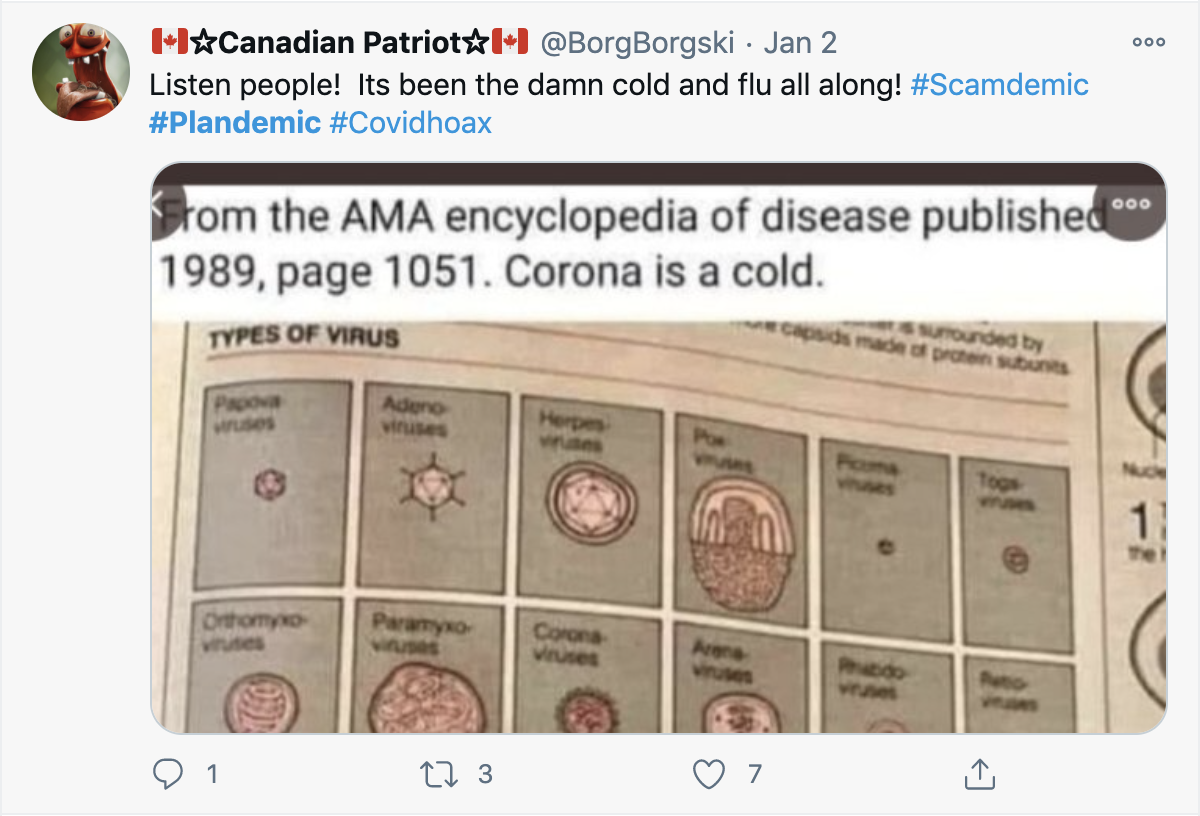
\includegraphics[width=14cm]{twitter_example.png}
  \caption{Příklad potenciálně dezinformačního tweetu, zdroj: vlastní tvorba}
  \label{fig:twitter example}
\end{figure}
\vspace*{-5mm}

\begin{framed}
{\small S ohledem na rozsah práce bohužel není možné udělat obsáhlejší analýzu, ta by musela být postavena nad větším množstvím dat, nicméně je na výše uvedeném obrázku možné ilustrovat, jak může vypadat jednodušší dezinformační tweet.}
\end{framed}

Po zadání jakéhokoliv z výše uvedených hashtagů je možné nalézt tisíce dezinformačních a misinformačních tweetů. Při omezení vyhledávání pouze na dnešní den jsem nalezl na Twitteru více než 500 tweetů s hashtagem \textit{\textbf{\#}scamdemic}. Při rozšíření vyhledávání na 3 dny je možné podívat se i na vývoj dosahu tohoto hashtagu, a to například za použití služby tweetbinder (ta bohužel v každém hledání omezuje počet tweetů na první stránku, reálný rozsah je tedy ještě mnohonásobně větší).\\

\begin{figure}[htbp]
  \centering
  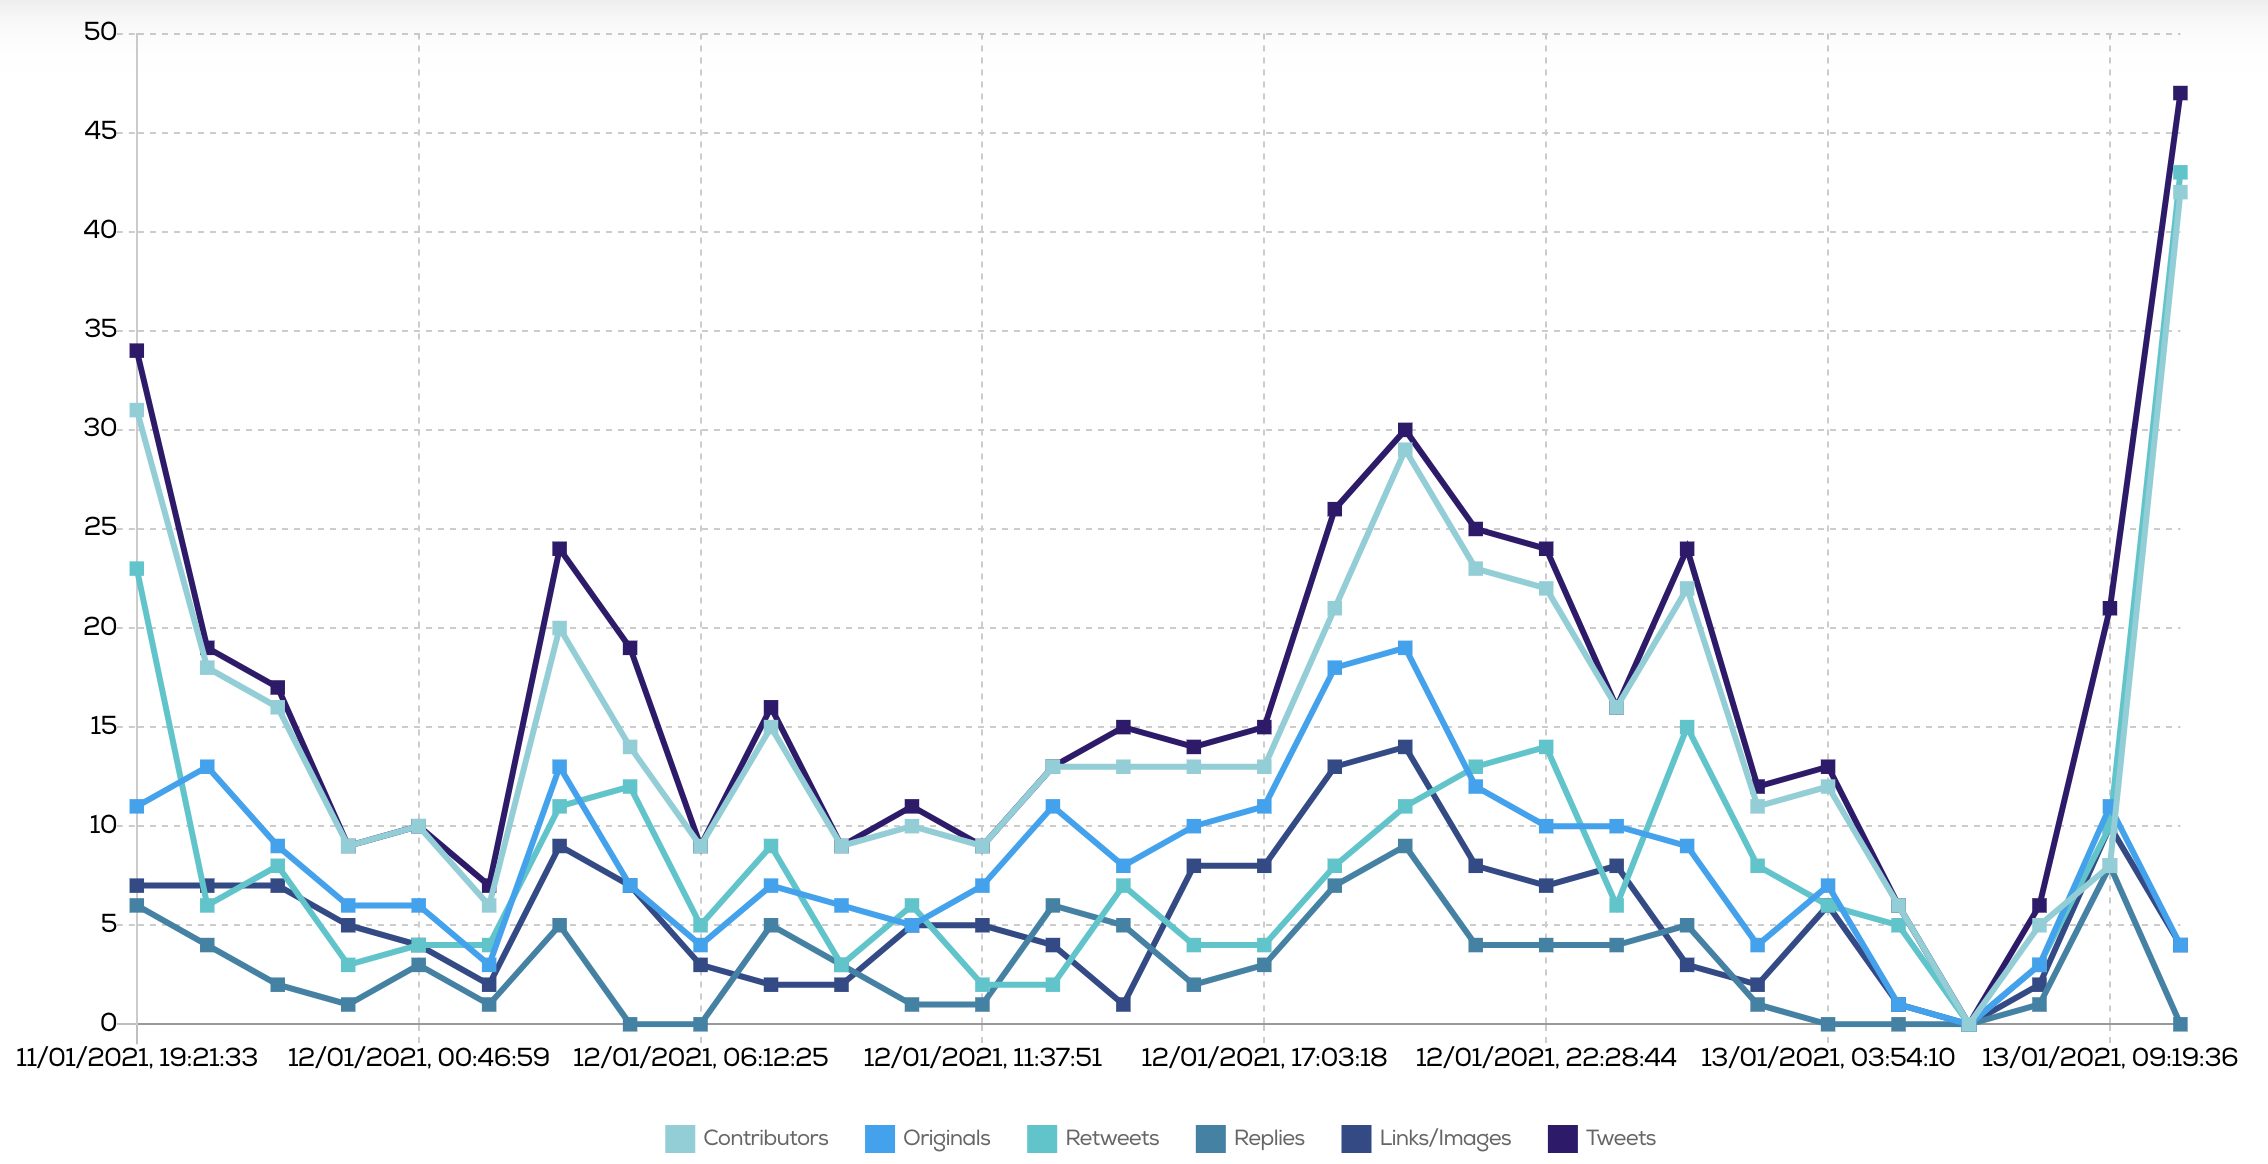
\includegraphics[width=14cm]{dosah.png}
  \caption{Vývoj dosahu \textit{\textbf{\#}scamdemic}, zdroj: tweetbinder}
  \label{fig:twitter dosah}
\end{figure}

Výše ilustrovaná dezinformace se možná na první pohled nemusí zdát natolik závažná, i kvůli menšímu počtu reakcí, v minulosti jsme však byli svědky mnoha případů, kdy vysoce postavení lidé s velkou základnou sledujících sdíleli při nejmenším misinformace. Jako příklad může posloužit Donald Trump, který, ačkoli na jeho obranu nutno dodat nepřímo, zmiňoval snahu o "zabití" viru za pomoci bělidla, které by mělo být podáváno nitrožilně\cite{noauthor_coronavirus_2020}. Je pak snadné si představit jak velký dosah může takováto misinformace mít a jak velkou újmu může způsobit.\\

%Samozřejmě pro odpovídající výsledek, by musel být dataset mnohem větší, toto bylo pouze pro ilustraci.\\

Rozsáhlejší průzkum zaměřený na Twitter a jeho používání jako platformy k šíření dezinformazí je například: \textit{An Exploratory Study of COVID-19 Misinformation on Twitter} od Gautam Kishore Shahi, Anne Dirkson a Tim A. Majchrzak, kteří svoji analýzu postavili na několika tisících vzorků\cite{shahi_exploratory_2020}, hlavní alarmující zjištění je, že vytvořený dezinformační tweet se v průměru šíří velikou rychlostí, tedy i tak "na první pohled neškodný" tweet, který jsem jako příklad uvedl výše, může cirkulovat mezi mnoha lidmi a potenciálně tedy i způsobit velkou újmu.\\

%Jako doklad mého tvrzení pak může sloužit například výzkum: https://arxiv.org/pdf/2005.05710.pdf, který dělal analýzu i na základě klasických klíčových slov, jako: \textit{\textbf{\#}covid19}, či \textit{\textbf{\#}coronavirus}.\\

%Další české dezinformační weby, sputnik

%\textbf{Výsledek:}
\subsection{Google Trends a dezinformace}

Rovněž je hypotézu možné ověřit prostřednictvím stránky Google Trends, do které lze zadat stejná klíčová slova a podívat se na frekvenci jejich vyhledávání.\\

Rozhodl jsem se v porovnání využít 3 klíčová slova, respektive slovní spojení, přičemž dvě jsou náchylná k využití k \textbf{dezinformačnímu obsahu} a jedno k \textbf{informačnímu obsahu}:\\

\begin{enumerate}
\item \textit{scamdemic} - \textbf{dezinformační},
\item \textit{end the lockdown} - \textbf{dezinformační},
\item \textit{protect others} - \textbf{informační}.	
\end{enumerate}
\vspace*{5mm}

\textbf{Výsledek, Obrázek č.~\ref{fig:google trends}:}

\begin{figure}[htbp]
  \centering
  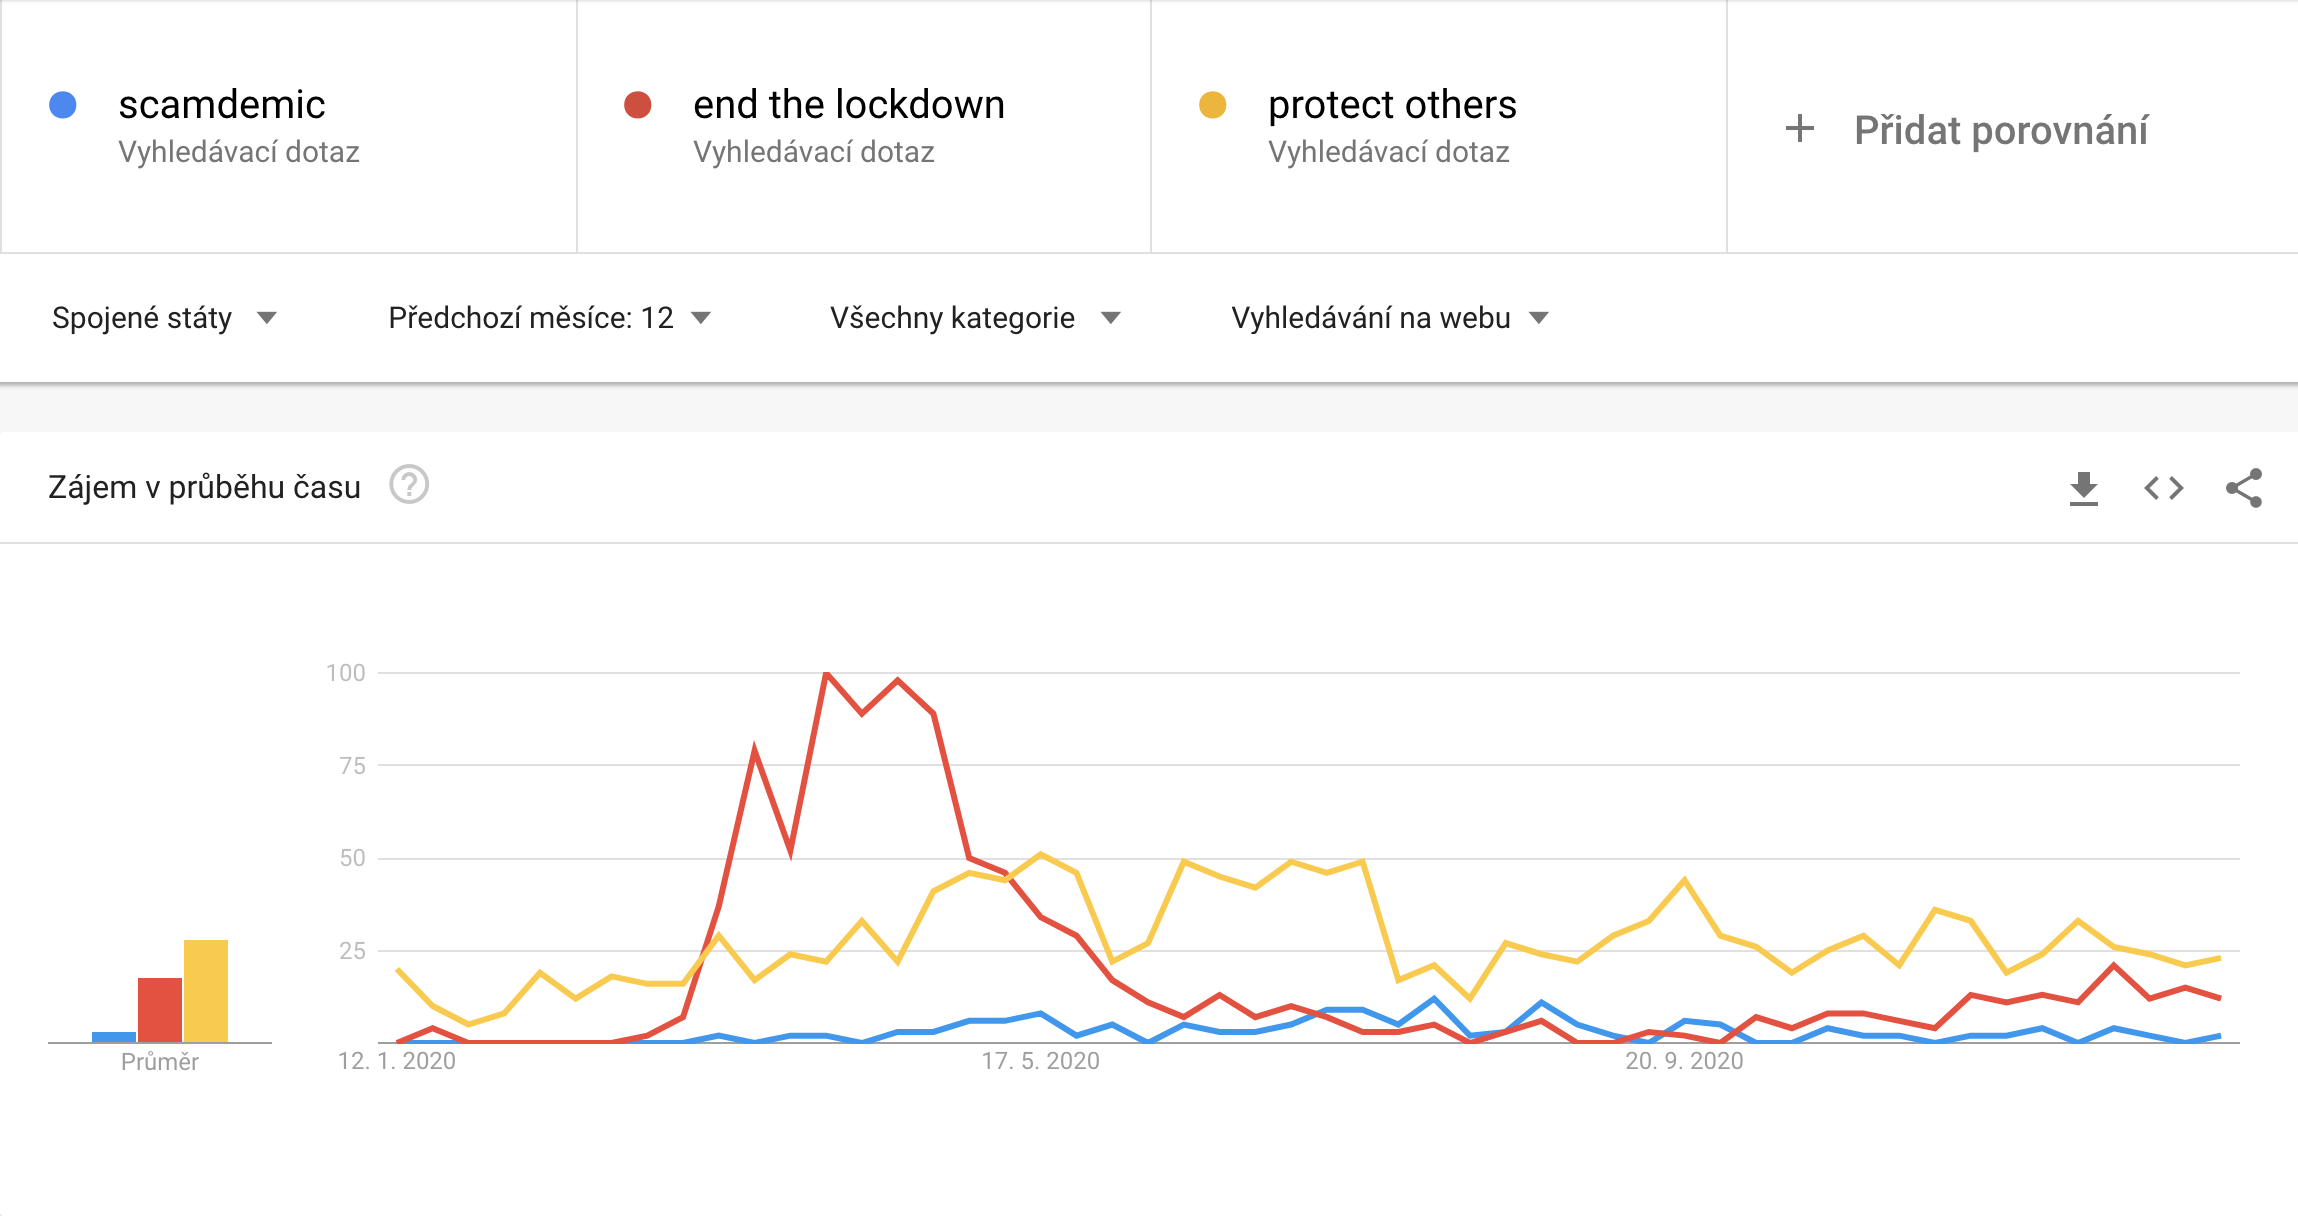
\includegraphics[width=14cm]{google_trends_analysis.png}
  \caption{Výsledek porovnání několika slovních spojení, zdroj: Google trends}
  \label{fig:google trends}
\end{figure}

Je možné pozorovat, že přes fakt, že pozitivní výraz \textit{protect the others} má v celém časovém období větší medián počtu vyhledávání, na začátku pandemie ho heslo \textit{end the lockdown} v počtu vyhledávání hravě předčilo, přičemž v poslední části grafu na něj nebezpečně znovu dotahuje, odhaduji, že především kvůli nechuti lidí řídit se dále vládními nařízeními a doporučeními kvůli délce trvání pandemie.\\

\newpage

Při zadání samotného hesla do vyhledávače od Googlu je možné dojít k následujícím závěrům:\\

\begin{centering}
\begin{tabular}{l|c}
 \textbf{Vyhledávané heslo} & \textbf{Počet vyhledaných výsledků} \\ 
\hline
\hline
 \textit{scamdemic} & 1,270,000 results \\  
 \textit{end the lockdown} & 537,000,000 results \\
 \textit{protect others} & 1,420,000,000 results \\
\hline
\hline    
\end{tabular}
  \captionof{table}{Výsledné počty odkazů k vyhledávaní jednotlivých slovních spojení, zdroj: Google vyhledávač}
  \label{tbl:odkaz}
\end{centering}
\vspace*{5mm}

Například množství odkazů, které vyhledávač od Google zobrazí po zadání hesla \textit{end the lockdown} je více než pět set milionů, je možné důvodně předpokládat, že potenciál výskytu dezinformačního obsahu mezi takovýmto množstvím výsledků bude obrovský.\\

Při porovnání grafu s tabulkou je vidět korelace mezi počtem vyhledávání a množstvím výsledků, z čehož dovozuji, že si subjekty publikující dezinformace úmyslně vybírají více užívaná hesla, samozřejmě tento bod je k diskuzi, neboť samotná korelace neznamená kauzalitu.\\

\begin{framed}
{\small Je nutné zmínit, že se jedná o povrchnější analýzu, která v žádném případě není průkazná a slouží pouze pro přestavu o potenciální možnosti rozsahu dezinformačního obsahu. Pro průkaznou analýzu by byl nutný další výzkum provedený společně s odfiltrováním důvěryhodných informací týkajících se dezinformací od faktických dezinformací, pro získání odpovídajících čísel, nicméně domnívám se, že pro ilustraci, kolik dezinformačního obsahu se v online prostoru může nacházet, a jak úrodná je pro tento obsah s ohledem na momentální situaci půda je při nejmenším zajímavá.}
\end{framed}

\newpage

\section{Jak proti dezinformacím bojovat?}

Jak je zřejmé z výše uvedeného, dezinformace představují velkou hrozbu, jak se proti nim ale účinně bránit?\\

Již v úvodu, při definování pojmu dezinformace, jsem zmínil, že dezinformace jsou nejvíce šířeny přes internet, a to zejména přes sociální sítě (problém mohou představovat zejména nemoderované sociální sítě jako například \textbf{Parler}), proto je zásadní, aby se velkou měrou o snahu vymítit dezinformace zasadili technologické společnosti jako Facebook, Twitter, Apple či Google a Microsoft, v českém prostředí by se měl zasadit o boj proti dezinformacím například Seznam, zejména pak při indexování webových stránek ve svém vyhledávači (a to tím, že dezinformační weby by nebyly indexovány).\\

Pozitivní je fakt, že snaha o boj proti dezinformacím se v poslední době stala pro tyto technologické giganty prioritou, proto reagují na dezinformace propagováním autoritativního obsahu, sdílením důvěryhodných informací od důvěryhodných zdrojů (vládní a nadnárodní zdravotnické agentury a to jak obecně tak i se zaměřením na vyhledávání těchto témat, tedy například při vyhledávání informací o Covid-19) a větší manuální i automatizovanou kontrolu sdíleného obsahu spojeného s takzvaným \textit{tagováním} potenciálně dezinformačního obsahu společně s jeho mazáním a blokací zdrojů, ze kterých tyto informace pocházely. Další obranná linie pak byla zavedena na úrovni snahy o zabránění automatického vytváření a šíření dezinformačního obsahu dávkově, tedy bez přičinění člověka primárně za pomoci botů, to vedlo, a dovoluji si tvrdit, že i v budoucnu bude vést k nutnosti reálné autorizace uživatelů platforem\cite{braidma_tackling_2017}.\\

\begin{figure}[htbp]
  \centering
  
\includegraphics[width=14cm]{this_claim_is_disputed.png}
  \caption{Takto může například vypadat \textit{otagování} dezinformačního příspěvku, zdroj: Twitter}
  \label{fig:disputed_claim}
\end{figure}

Současná krize a koordinovanější přístup technologický společností vedl ke změně pravidel užívání jednotlivých platforem vztahujících se především k šíření nepravd a polopravd a potenciální možnosti toho, že toto sdílení může vyvolat mnoho škod a dá se tak, alespoň s malým oddechem, počítat s tím, že takto nastolený nový přístup budou technologické společnosti a i klasická média držet i do budoucna.\\

%\newpage

Zatímco moderování předdefinovaného obsahu, který je zřejmě škodlivý, a to zejména s ohledem na fyzickou újmu, tedy například propagace perorálního požívání čístících prostředků jako prostředku k léčbě Covidu-19 je poměrně jednoduchá, minimálně v menší škále, a lze mnohakdy zachytit automatizovaným způsobem, řešení dezinformací při vznikající, respektive nově vzniklé/objevené pandemii je s ohledem na mnoho neznámých složité (o nově vzniklém viru nemusí být v jeho prvopočátcích mnoho informací). Je tak složitější odhalit přímé dezinformace, neboť i oficiální a důvěryhodné zprávy se ve svých prvopočátcích nemusí opírat o množství jiných důvěryhodných zdrojů, a to zejména pokud určitým aspektům nové nemoci vědci při jeho objevení ze začátku nerozumí, to se ostatně stalo i v případě momentálně probíhající pandemie koronaviru, otázka v oblasti veřejného zdraví může být dále značně zpolitizována a podléhat častým změnám. Koncept prvního bodu stanoveného \textbf{WHO} (viz první kapitola) je tak složitější naplnit, stejně tak jako je složitější určit, jaké příspěvky mohou svojí informační/dezinformační povahou způsobit společnosti újmu.\\

Je proto logické, že si mnoho lidí pokládá stejnou otázku, kterou jsem vyslovil na začátku této kapitoly, tedy otázku \textit{"Jak vlastně proti dezinformacím máme bojovat?"}. Je nutné vzít v potaz několik zásaních otázek, které jsou doplňující k pohledu \textbf{WHO} na dezinformace:\\

\begin{enumerate}
\item Jakým způsobem by společnost jako celek i jednotlivci měli reagovat na šíření dezinformací/misinformací v případech, kdy o tématice není v danou chvíli mnoho informací, vědecká shoda a výzkum, jaké informace by tedy měly být propagovány, a jaké naopak netolerovány?
\item Jakým způsobem by společnost jako celek i jednotlivci měli přistupovat k, a čelit, dezinformacím v různých podobách?
\item Jaké podoby by měli být prioritizovány, mělo by se s veškerými dezinformacemi zacházet stejně (otázky, pochybné důkazy, vizualizace - obrázky, videa), tedy všechny hodnotit jako kategorii přímých nepravdivých či zavádějících tvrzení na základě jejich vnímaného záměru, či jejich potenciálních důsledků spočívajících primárně v možnosti způsobit újmu?
\item Po zodpovězení předchozích 3 bodů (jakožto k rozšíření bodu prvního vyslovené v první kapitole ze strany \textbf{WHO}, jaká by měla být nejefektivnější strategie pro zmírnění dopadu dezinformací a jejich následného vymícení jak v online, tak i v offline prostoru? 
\end{enumerate}
\vspace*{5mm}

Po zodpovězení prvních 3 (1) otázky tedy nastává ta nejdůležitější otázka, na kterou hledáme jako společnost odpověď, jaká strategie je k vymícení dezinformací nejvhodnější, hledáme tedy odpověď na otázku \textbf{"JAK"}?\\

Již na začátku této kapitoly jsem nastínil způsoby, které používají technologické společnosti pro boj s dezinformacemi v online prostoru,  např. odstranění, snížení viditelnosti, \textit{otagování}, zavedení možnosti nahlášení. Komplexní obrana namířená přesně proti nově vznikajícím dezinformačním hrozbám tak ve svém výsledku, vzhledem k výše vyřčenému, může být komplikovaná ve velkém měřítku nejen díky masivním komunitám a velké diverzifikovanosti příspěvků a hesel, ale i vzhledem k rychlosti šíření dezinformací (viz zdroj ohledně rychlosti šíření dezinformací) v reálném čase.\\

Všechno řešení ale nespočívá jen v technologické sféře, potřeba ověřovat si informace a kritické myšlení společně s co největší informovaností musí být rozvíjeno i na individuální úrovni, což je konečně to, co může přispět k vymícení dezinformací, zatímco editační snahy (zmíněné výše) v online a offline zdrojích mohou pomoci, nejsou samospásné, finální fronta proti dezinformacím musí být individuálně u každého člověka. V individuální sféře každého člověka je tak vždy potřeba posilovat především vzdělání, osvětu a kritické myšlení.\\

U lidí, kteří jsou dezinformacemi ovlivněni se však můžeme setkávat i s argumentem, že snaha bojovat proti dezinformací (Twitter například dezinformační příspěvky maže, nebo k nim připojuje vysvětlivky, viz Obrázek č.~\ref{fig:disputed_claim}) se ve své podstatě rovná cenzuře, a že všechny názory by se měly tolerovat. Je tak podstatné nalézt odpověď i na tuto problematiku, aby společnost tomuto názoru dokázala s dostatečnou precizností obstát.\\

\newpage

Troufám si tvrdit, že dobré vysvětlení, proč není možné boj proti dezinformacím považovat za cenzuru poskytu následující grafika Obrázek č.~\ref{fig:tolerance_paradox}:\\

\begin{figure}[htbp]
  \centering
  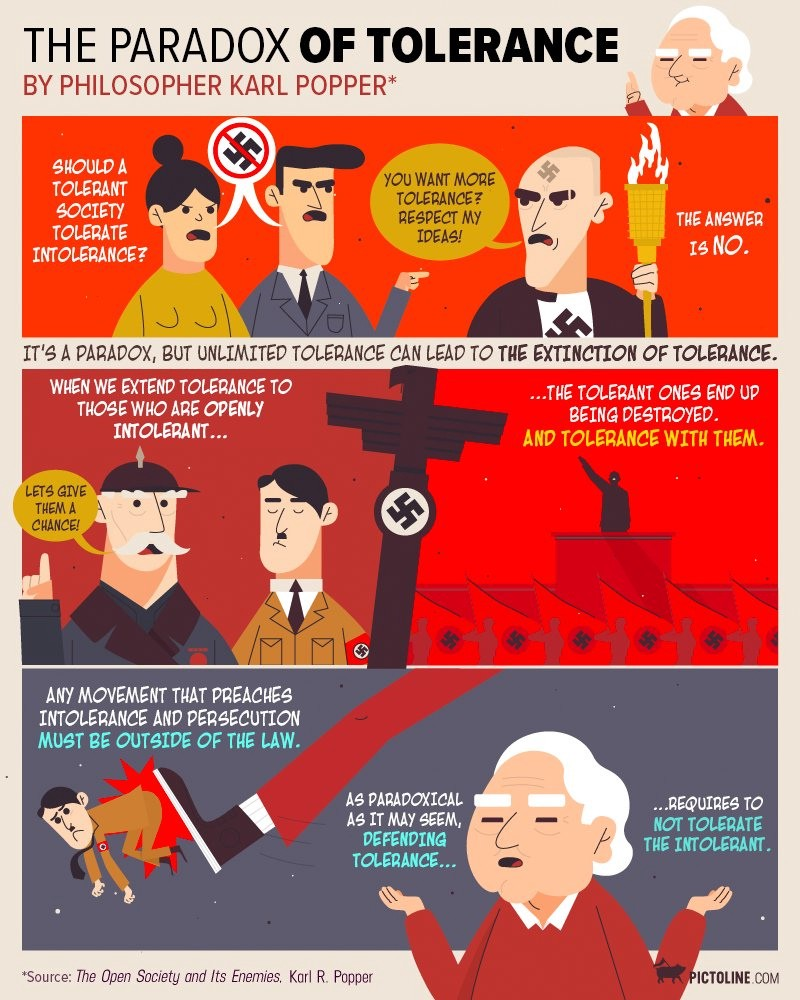
\includegraphics[width=12cm]{intolerance_vs_tolerance.jpeg}
  \caption{Paradox tolerance (Pictoline.com)}
  \label{fig:tolerance_paradox}
\end{figure}

Diskuze o paradoxu tolerance je důležitá právě ve vztahu k dezinformacím, neboť ty jsou často chráněny pod heslem \textit{"svoboda projevu"}, zde se objevuje i tento jakýsi \textit{"informační paradox"}, neboť absolutní svoboda projevu stejně tak, jako absolutní tolerance, vede k potlačení toho, na čem stojí, tedy svobodě projevu.\\

\subsection{Jak se mohu proti podlehnutí dezinformačním bludům bránit já, jako jednotlivec?}

Osobně jsem velkým zastáncem zjednodušených grafik, neboť ty často vyjadřují stovky až tísíce slov v jedné grafice. Jeden z nejzajímavějších informačních materiálů k této problematice, který se za poslední dobu objevil je infografika od Evropské komise, který shrnuje individuální obranu do 13 jednoduchých bodů:\\

% studijní materiál jak se bránit proti dezinformacím jako jednotlivec je například poskytnuto v následujícím článku ve stručných 13 bodech\cite{článek_nice}. :-) \\

\begin{figure}[htbp]
  \centering
  
\includegraphics[width=12cm]{misinformation.png}
  \caption{Takto může například vypadat \textit{otagování} dezinformačního příspěvku\cite{noauthor_13_nodate}}
  \label{fig:disputed_claim}
\end{figure}

\textbf{Body:}

Více info zde\cite{braidma_tackling_2017}.

\newpage

\section{Závěr}

Je zřejmé, že dezinformace představují velkou hrozbu pro moderní společnost, tato hrozba je v poslední době posílena i díky probíhající krizi, která zakládá živnou půdu pro jakékoliv dezinformační snahy.\\

S ohledem na nedávné události spojené například s volbami v USA můžeme vidět, kam až může šíření dezinformací zajít a k čemu může občany přimět.\\

Podobných dezinformačních snah si můžeme povšimnout i vzhledem k tématu světové pandemie, není tedy iluzurní myslet si, že jejich sdílení může vyůstit ve velice negativní následky. Ostatně dopad dezinformací je vidět v poslední době především k očkování, které je pro vyřešení krize klíčové. Cílová hodnota proočkování k překonání krize je 95\%\cite{noauthor_vaccines_nodate} obyvatelstva, dezinformace však mohou dosažení tohoto čísla značně ztížit a v konečném důsledku tak i v nejhorším možném případě zabránit, abychom se efektivně vypořádali s nákazou koronaviru\cite{middleton_information_nodate}. I nejen z toho důvodu je zásadní, abychom proti dezinformací ve všech oblastech důrazně vystupovali a bojovali za použití veškerých nám dostupných nástrojů.\\

Boj proti dezinformacím však není a nebude snadný, neboť mnohkdy nelze vyhodnotit duálně jako prostá pravda, či nepravda. Ke způsobu zvádnutí dezinformací je proto nutné vytvořit hloubější narativ, společně s důrazem na velkou odpovědnost klasickým médií a technologických společností, ve vztahu ke způsobu moderování obsahu, a nakonec i nás všech jako jednotlivců. Boj proti dezinformacím rovněž vyžaduje aktivní zapojení státních orgánů a dalších zodpovědných orgánů, u nichž je rovněž vyžadována absolutní transparentnost ve vztahu k tomu, co je známo a ktomu, co v danou chvíli ještě známo není. I následování výše vyřčených bodů může posloužit k utvrzení důvěry v důvěryhodné informace u jednotlivců, kteří jsou veřejným institucím, médiím a dalším organizacím spíše nakloněni, u jednotlivců, kteří vůči těmto orgánům a institucím mají hlubokou nedůvěru nemusí moderace obsahu a transparentnost výrazně změnit jejich hodnoty a postoje, v takovémto případě tedy bude nutné zodpovědně přistoupit především ke vzdělávání obyvatelstva a rozvíjení jejich kritického myšlení. Jedno však zůstává jisté, boj proti dezinformacím bude ještě bohužel běh na dlouho trať.
%\section*{Zadání}
Teorie systémů

\section{Úvod}
Lorem ipsum dolor sit amet, consectetuer adipiscing elit. Proin mattis lacinia justo. Curabitur bibendum justo non orci. Integer lacinia. Nullam faucibus mi quis velit. Nam libero tempore, cum soluta nobis est eligendi optio cumque nihil impedit quo minus id quod maxime placeat facere possimus, omnis voluptas assumenda est, omnis dolor repellendus. Aliquam ante. Duis viverra diam non justo. Nulla pulvinar eleifend sem. Aliquam in lorem sit amet leo accumsan lacinia. Ut tempus purus at lorem. Obrázek č.~\ref{fig:tux}

\begin{figure}[htbp]
  \centering
  
\includegraphics[width=6cm]{tux.png}
  \caption{Obrázek}
  \label{fig:tux}
\end{figure}

\section{Cíl práce a metodika}
Vivamus porttitor turpis ac leo. Cras elementum. Quisque porta. Proin pede metus, vulputate nec, fermentum fringilla, vehicula vitae, justo. Etiam ligula pede, sagittis quis, interdum ultricies, scelerisque eu. Phasellus faucibus molestie nisl. Duis risus. Morbi imperdiet, mauris ac auctor dictum, nisl ligula egestas nulla, et sollicitudin sem purus in lacus. Integer imperdiet lectus quis justo. Nam quis nulla. Cras elementum. Quisque tincidunt scelerisque libero. Maecenas lorem. Praesent vitae arcu tempor neque lacinia pretium. Cum sociis natoque penatibus et magnis dis parturient montes, nascetur ridiculus mus. Nulla quis diam. Duis condimentum augue id magna semper rutrum. Nulla non lectus sed nisl molestie malesuada.

\section{Teoretická část}

Vivamus porttitor turpis ac leo. Sed elit dui, pellentesque a, faucibus vel, interdum nec, diam. Duis viverra diam non justo. Etiam dui sem, fermentum vitae, sagittis id, malesuada in, quam. Nunc auctor. In enim a arcu imperdiet malesuada. Aenean fermentum risus id tortor. In enim a arcu imperdiet malesuada. Duis aute irure dolor in reprehenderit in voluptate velit esse cillum dolore eu fugiat nulla pariatur. Pellentesque pretium lectus id turpis. Etiam dui sem, fermentum vitae, sagittis id, malesuada in, quam. Fusce nibh. Pellentesque pretium lectus id turpis. Phasellus rhoncus. Etiam bibendum elit eget erat. Sed ut perspiciatis unde omnis iste natus error sit voluptatem accusantium doloremque laudantium, totam rem aperiam, eaque ipsa quae ab illo inventore veritatis et quasi architecto beatae vitae dicta sunt explicabo. Class aptent taciti sociosqu ad litora torquent per conubia nostra, per inceptos hymenaeos. Cum sociis natoque penatibus et magnis dis parturient montes, nascetur ridiculus mus. Tabulka č.~\ref{tbl:odkaz}

\begin{centering}
  \begin{tabular}{|c|c|}
    \hline
    1 & 2 \\
    \hline
    3 & 4 \\
    \hline
  \end{tabular}
  \captionof{table}{Krásná tabulka}
  \label{tbl:odkaz}
\end{centering}

\section{Praktická část}
Sed ac dolor sit amet purus malesuada congue. Duis pulvinar. Quis autem vel eum iure reprehenderit qui in ea voluptate velit esse quam nihil molestiae consequatur, vel illum qui dolorem eum fugiat quo voluptas nulla pariatur? Fusce wisi. Nunc auctor. Vivamus ac leo pretium faucibus. Ut enim ad minim veniam, quis nostrud exercitation ullamco laboris nisi ut aliquip ex ea commodo consequat. Sed convallis magna eu sem. Nullam rhoncus aliquam metus. Integer imperdiet lectus quis justo. Pellentesque habitant morbi tristique senectus et netus et malesuada fames ac turpis egestas. Fusce tellus. Curabitur sagittis hendrerit ante. Vestibulum fermentum tortor id mi. Etiam commodo dui eget wisi. Donec quis nibh at felis congue commodo. Nam sed tellus id magna elementum tincidunt.

\section{Výsledky a závěr}
Morbi imperdiet, mauris ac auctor dictum, nisl ligula egestas nulla, et sollicitudin sem purus in lacus. Cum sociis natoque penatibus et magnis dis parturient montes, nascetur ridiculus mus. Aenean placerat. Duis ante orci, molestie vitae vehicula venenatis, tincidunt ac pede. Fusce tellus. Etiam dui sem, fermentum vitae, sagittis id, malesuada in, quam. Duis condimentum augue id magna semper rutrum. Etiam neque. Maecenas lorem. In dapibus augue non sapien. Vestibulum fermentum tortor id mi. Nullam lectus justo, vulputate eget mollis sed, tempor sed magna. Nullam feugiat, turpis at pulvinar vulputate, erat libero tristique tellus, nec bibendum odio risus sit amet ante. Aenean id metus id velit ullamcorper pulvinar. Fusce dui leo, imperdiet in, aliquam sit amet, feugiat eu, orci. Pellentesque sapien. Maecenas lorem. Fusce dui leo, imperdiet in, aliquam sit amet, feugiat eu, orci.


% === Bibliography list, ordered alphabetically ===
\phantomsection % PDF list links
\addcontentsline{toc}{section}{Seznam použitých zdrojů}
\renewcommand{\refname}{Seznam použitých zdrojů}

\bibliographystyle{unsrt} %acm czplain
\bibliography{out}

\end{document}
